En premier lieu j’ai commencé par regarder quel bibliothèques pouvais remplir mes besoins de reconnaissance faciale en Python. 
Pour ce sujet j’ai retenu 2 bibliothèque principales :
\begin{itemize}
    \item La première est OpenCV qui possède les fonctions afin de faire de la reconnaissance facial. C’est une bibliothèque éprouvé et dont de nombreux sujet font allusion sur Internet.
    \item La deuxième est GluonCV qui propose les mêmes fonctionnalités, mais qui à l’avantage de proposer un large choix d’IA près entrainé. Cependant elle est plus récente et les sources à son sujet sont plus rares.
\end{itemize}

\begin{figure}[h]
    \centering
    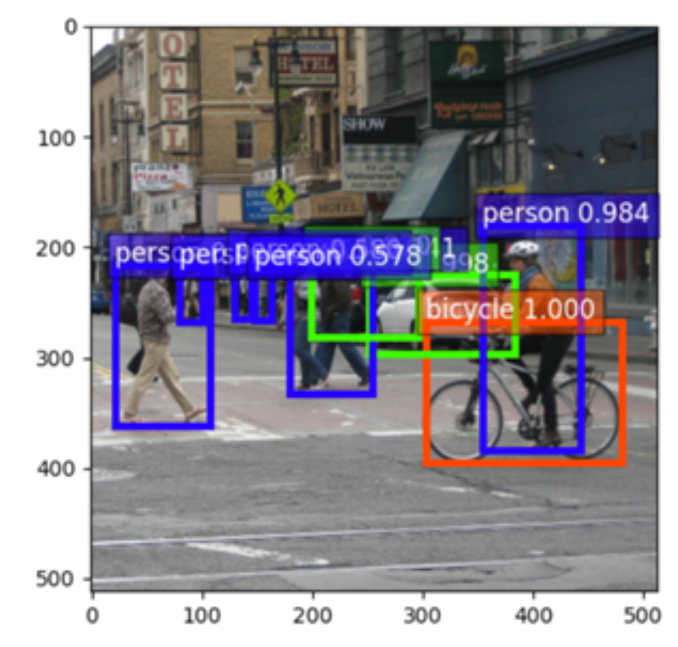
\includegraphics[width=.8\linewidth]{Figures/GluonCV_start.png}
    \caption{Le "Hello word" de GluonCV qui identifies des passants dans la rue grâce à une IA}
\end{figure}

Cependant la technologie python n’est pas la seule à proposer des solutions de reconnaissance faciale. En plus de cela sont intégration à une page web n’est pas simple.
Le javascript avec Node.js propose aussi de nombreuses solutions qui utiliserons des API mises à disposition par de grandes entreprises afin de faire de la reconnaissance faciale.
Api utilisables :
\begin{itemize}
    \item TensorFlow :
\end{itemize}



